% USE PDFLatex!
% to correctly render Swedish characters

\documentclass{popsci}

\usepackage[utf8]{inputenc}
\usepackage[swedish, english]{babel}

\usepackage{fancyhdr}
\usepackage{titling}
\usepackage{color}
\usepackage{colortbl}
\usepackage{graphicx}
\usepackage{flushend}
\usepackage{lmodern}


% Please specify the presentation date
\presentationsdag{2020-06-11}

% use either of these commands to specify the title of your thesis
 \examensarbete{Cross-lingual toxicity classification}
% To create a title in two rows, leave examensarbete blank and fill in examensarbeteTwoRows.
%\examensarbeteTwoRows{Cross-lingual toxicity classification}{Synthesizeable Model Supporting Design Space Exploration}
\student{Malte Kauranen}
\supervisor{Pierre Nugues (LTH)}
\examiner{Jacek Malec (LTH)}

% Your pop-sci title should be different (more catchy) than your thesis title
\title{Flerspråkig identifikation av hatiska texter}


\begin{document}

% not more than 4 rows!
\theabstract{Diskussioner online blir allt viktigare för vårt samhälle men plågas ofta av en hätsk stämning. Det här arbetet undersöker om man kan bygga automatiska system som hittar hatiska kommentarer på tidningar som kan användas för flera språk samtidigt.}%Applikations-specifika processorer är allt mer vanligt för få ut rätt prestanda med så lite resurser som möjligt. Detta arbete har en parametrisk modell för att kunna testa hur mycket resurser som behövs för en specifik applikation.}


{\noindent Tidigare i historien har människor varit tvungna att passivt motta media utan en möjlighet att interagera med det själv. Med framväxten av sociala medier har vi kommit ett steg närmre att inte bara konsumera media men faktiskt interagera med det. Vi kan öppet och fritt diskutera med nästan alla människor på jorden på vissa plattformar. På till exempel Twitter kan man inte bara följa och läsa vad andra skriver utan även svara på dem så att vem som helst kan läsa det.

Många tidningar har för att följa med i den tekniska utvecklingen försökt göra det möjligt för läsare att kommentera på tidningar. Hoppet har varit att användare ska bidra med ny intressant information för läsarna, men också att användarna ska bli mer lojala till tidningen. Tyvärr händer det här sällan i praktiken och diskussionen slutar ofta i smutskastning och förolämpningar. Det här rimmar inte bra med läsarnas förväntningar på tidningen. För att tidningen ska tillåta att gemene man deltar i diskussion måste nivån på diskussionen vara hög och till exempel rasism och förolämpningar nästan obefintliga. Det är just det här problemet som det här arbetet försöker lösa.

Tillsammans med Ifrågasätt som säljer en kommentarsfältslösning till tidningar har jag tagit fram ett automatiserat system som kan hitta hatiska texter. Systemet är inte perfekt och kommentarerna behöver fortfarande läsas av människor för att verifiera att de inte är hatiska, men det är ett kritiskt verktyg för att prioritera vilka kommentarer som moderatorerna ska läsa först. Systemet hittar nästan alla icke-hatiska kommentarer och få hatiska misstas för icke-hatiska. Med hjälp av systemet kan alltså Ifrågasätt se till att hatiska kommentarer försvinner mycket snabbare från deras plattform. Undersökningar visar också att det här systemet väldigt lätt kan utökas till andra språk. I en startfas behövs inte ens data för nya språk som det ska implementeras i. Men efterhand när moderatorerna markerar texter som hatiska i det nya språket blir prestandan snabbt lik den för bara ett språk.

Det finns dock vissa problem med datan som användes. En undersökning av datan som moderatorerna på Ifrågasätt har skapat visar att moderatorerna inte alltid har samma åsikt om vad som är en hatisk kommentar. Eftersom den här datan användes för att träna modellerna så kan modellerna inte heller ha en konsekvent bild av vad som är en hatisk text. Jämförelser med annan data visar att förbättringar av moderatorernas samstämmighet sannolikt skulle förbättra prestanda och göra moderatorernas jobb i framtiden lättare.

%För att kunna välja vilken typ av processor som är rätt för den specifika applikationen krävs det ofta att man snabbt kan testa olika prototyper. Att implementera dessa till hårdvara kan ofta vara tidskrävande och ifall det visar sig att implementationen inte klarar dem kraven man ställt för prestanda och energieffektivitet, måste man designa för nya parametrar och mer tid har blivit slösat. %Om den här processen istället kan göras automatiskt utifrån dessa design-parametrar kan man teoretiskt spara en massa tid.

%\begin{figure}[!bth] % Use pictures in your pop-vet!
%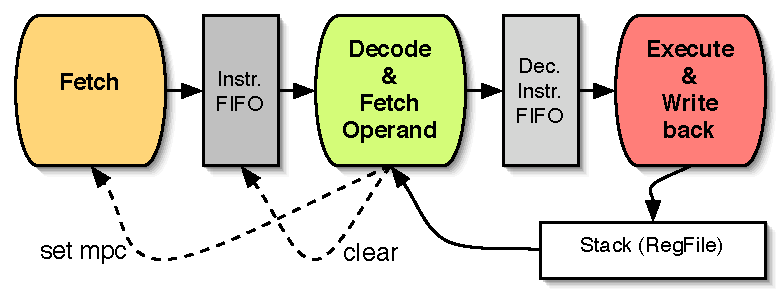
\includegraphics[width=\columnwidth]{samplePic.pdf} 
%\caption{En fin bild}
%\end{figure}
%}

\end{document}
